\section{Numerical results\label{sec:numres}}

In this section, numerical simulations are used to assess the
performance of the MFD solver in solving the quasi-static force-free
model (Equations~\eqref{eq:4.565}--\eqref{eq:4.580}) with different
configurations.  The simulations were run on NERSC's Cori and
Perlmutter machines.

\noindent Cori is a Cray XC40 with a peak performance of about 30 petaflops and
is comprised of 2388 Intel Xeon "Haswell" processor nodes and 9688
Intel Xeon Phi "Knight's Landing" (KNL) nodes. 
On Cori, the computations were carried out on Haswell Compute Nodes: Each node has two sockets, each
socket is populated with a 2.3 GHz 16-core Haswell processor (Intel
Xeon Processor E5-2698 v3). Each core supports 2 hyper-threads, and
has two 256-bit-wide vector units. The theoretical peak is 36.8
Gflops/core, 1.2 TFlops/node and 2.81 PFlops total. Each node has 128
GB of DDR4 2133 MHz memory (four 16 GB DIMMs per socket) for a total
aggregate memory of 298.5 TB. For our computations on Cori, we used 4 Haswell
nodes for a total of 128 cpus.

\noindent Perlmutter is a Cray EX supercomputer comprising 3072 CPU-only and 1536 GPU-accelerated nodes and has a performance of 3-4 times Cori. 
On Perlmutter, the computations were run on CPU-only nodes: each nodes is populated with two 2.45GHz 64-core AMD EPYC 7763 processors. 
The theoretical peak is 39.2 Gflops/core, 2.52 TFlops/socket and 7.7 PFlops total. Each node has 512 GB of DDR4 memory for a total aggregate memory of 1536 TB. In our computations, we used 4 Haswell nodes for a total of 128 cpus.
For our computations on Perlmutter, we used 1 CPU-only node for a total of 128 cpus.

% Talk about PETSc (references 34-36 can be found https://aip.scitation.org/doi/pdf/10.1063/1.2838244, and there are more referenes on PETSc's webpage)
\noindent
For parallelization, we employ the Parallel Extensible Toolkit for
Scientific computing (PETSc) library \cite{petsc-web-page,
  petsc-user-ref, petsc-efficient}.
% Cite TS component of PETSc 
For the time-integration, we rely on PETSc's TS library that provides a framework for the scalable solution of ODEs and DAEs arising from the discretization of time-dependent PDEs \cite{AbhyankarEtAl2018}.
The list of available methods comprises, inter alia, IMEX Runge-Kutta schemes, Forward and Backward Euler, Crank-Nicolson,  Rosenbrock W-schemes and GL schemes with global error estimation.
We also use the DMSTAG component of PETSc for "staggered grid" representation. This allows the degrees of freedom to be associated with all "strata" in a logically-rectangular grid, i.e., elements, faces, edges, and vertices.

% Talk about the mesh resolution
\noindent
Simulations are run for a cylindrical mesh that has a resolution of
$100 \times 2 \times 200$, i.e. 100 cells in r direction, 2 cells with
periodic boundary conditions in $\phi$ direction and 200 cells in z
direction.
% Cite DMStag component of PETSc


\noindent The numerical results are organized into five sections.

\subsection{Computing the effective resistivity of ITER vacuum vessel}

The ITER tokamak reactor has an interesting engineering design in
which the vacuum vessel is to carry the inductive toroidal current as
the response to a dynamically evolving plasma, such as that during a
VDE after a thermal quench.  To enable this, the blanket modules,
which are attached to the vacuum vessel and face the plasma, are
insulated from each other along the toroidal direction so no net
toroidal current is allowed in the blanket modules.  To model the
plasma VDE properly, one must properly account for the image current,
especially the toroidal one, in the vaccum vessel.  The actual ITER
vaccum vessel has complicated structures and a hollow interior for
neutron moderating inserts, the details of which are not necessary in
the usual plasma modeling. The essential property of the vacuum vessel
for plasma modeling is its characteristic time for a wall current to
decay in the absence of a plasma inside the chamber.  This so-called
wall time of the vacuum vessel, $\tau_{VV} \equiv L/R,$ is the ratio
of inductance $L$ and resistance $R$ of the metal structure. The
inductance $L$ is set by the geometry of the conducting structure,
while $R$ has seperate toroidal and poloidal values, corresponding to
the decay of a net toroidal and a poloidal current in the vacuum
vessel. For wall feedback on VDEs, the toroidal one is most important,
and for ITER, the toroidal wall time is known to be around \SI{500}{\milli\second}. The
geometric simplification of the vaccum vessel, shown in light blue
(value of -1 for the levelset function) in Figure~\ref{fig:5layer},
implies that the correct $\tau_{VV}=$~\SI{500}{\milli\second} can be recovered by an
effective electric resistivity $\eta_{VV}$ for the vacuum vessel that
would be somewhat diffierent from the $\eta$ of the stainless steel
that is used to construct the vacuum vessel.  This effective
$\eta_{VV}$ is directly computed here to match a given $\tau_{VV}$ as
follows.

The goal here is to consider an isotropic vacuum vessel with uniform
resistivity, and find the resistivity value that would yield the
targetted wall time for ITER setting (around \SI{500}{\milli\second}). For that
purpose, we run initial tests for the magnetic diffusion problem where
we take the same high resistivity value (to mimic a vacuum response)
for all the computational domain except the vacuum vessel, and a lower
resistivity value for the vacuum vessel $\Omega^{V}$. The initial
magnetic field has to be set such that the current is nonzero only in
the vacuum vessel. We recall that the magnetic field in the tokamak
can be represented by
\begin{equation}
{\B} = \nabla \phi \times \nabla \psi + g_0 \nabla \phi, 
\label{eqn:Bfrompsi}
\end{equation} 
where $\psi$ is the poloidal flux function and $g_0$ is a scalar constant. 

Enforcing a magnetic field such that the current is nonzero only in
the vacuum vessel amounts to solving the fixed-boundary problem
\begin{equation}\label{eq:fixedbdeq}
  \begin{aligned}
    \frac{1}{\mu_0 r} ~ \Delta^{*} \psi & = J_0 && \text{in} \quad \Omega^{V}, \\
    \frac{1}{\mu_0 r} ~ \Delta^{*} \psi & = 0 && \text{in} \quad \Omega \setminus \Omega^{V}, \\
    \psi & = 0,&& \text{on} \quad \partial \Omega;
  \end{aligned}
\end{equation} 
where the toroidal elliptic operator is defined as   
\begin{equation}
\Delta^* \psi := \dfrac{\partial^2 \psi}{\partial r^2}-\dfrac{1}{r}\dfrac{\partial \psi}{\partial r}+ \dfrac{\partial^2 \psi}{\partial z^2},
\end{equation}
After solving the problem~\eqref{eq:fixedbdeq}, and computing the
magnetic field with~\eqref{eqn:Bfrompsi}, we obtain the current shown
in Figure~\ref{fig:5-layer_J0}.
\begin{figure}[ht]
\begin{center}
\includegraphics[width=\textwidth]{curlB.png}
\caption{The curl of the initial magnetic field in $\mathbf{e}_{\phi}$ direction.} 
\label{fig:5-layer_J0}
\end{center}
\end{figure} 
With a resistivity value of $\eta_{\rm VV} = \SI{1e+3}{\ohm\meter}$
(i.e. a Lundquist number $S_{\rm VV} = \num{2.7646e-2}$) inside the
vacuum vessel if the resistive diffusion time is normalized by the
plasma Alfven time) and $\eta = \SI{1e+6}{\ohm\meter}$ ($S =
\num{2.7646e-5}$) elsewhere, we obtain the current evolution depicted
in Figure~\ref{fig:current_VVdiffusion_S2e-2_2e-5_time}.  The slope
%at $t=0$ is equal to:
\begin{equation}
a_1 := \dfrac{\ln(10^5) - \ln(10^6)}{\num{3e-9} - \num{1.5e-9}} = \num{-1.53e+9}.
\end{equation}
\begin{figure}[!h]
\centering
\begin{subfigure}[b]{0.5\textwidth}
\centering
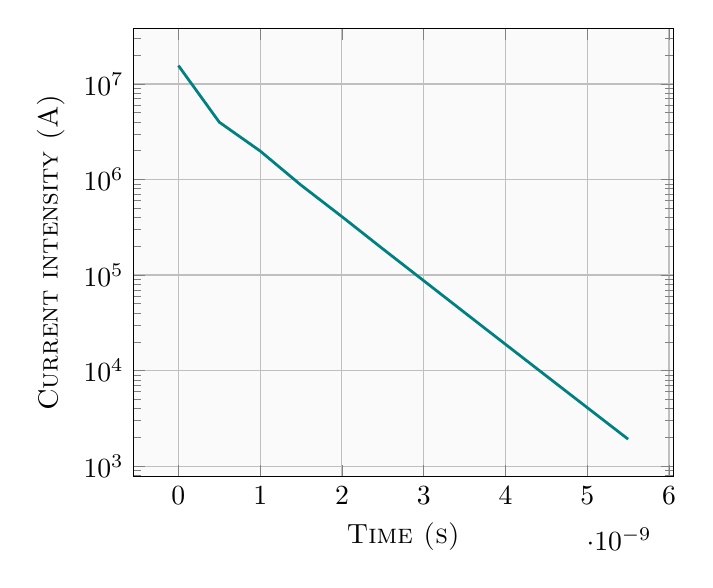
\begin{tikzpicture}[scale=1,>=latex]
\begin{axis}[ymode=log, xlabel=\textsc{{Time (s)}}, ylabel=\textsc{{Current intensity (A)}}, ymajorgrids, xmajorgrids, axis background/.style={fill=gray!4},, legend style={legend columns=2,at={(0.5,-0.2)},anchor=north}]
\addplot+[color=teal,line width=1pt,mark=none] coordinates {(0, 1.55782e+07) (0.5e-9, 3.97973e+06) (1e-9, 1.9874e+06) (1.5e-9, 872492) (2e-9 , 408238) (2.5e-9, 187740) (3e-9, 87194.3) (3.5e-9, 40461.7) (4e-9, 18828.8) (4.5e-9, 8771.88) (5e-9, 4092.83) (5.5e-9, 1911.82)};
\end{axis}
\end{tikzpicture}
\caption{$\eta_{\rm VV} = 10^3 ~\SI{}{\ohm\meter}$}
\label{fig:current_VVdiffusion_S2e-2_2e-5_time}
\end{subfigure}%
~
\begin{subfigure}[b]{0.5\textwidth}
\centering
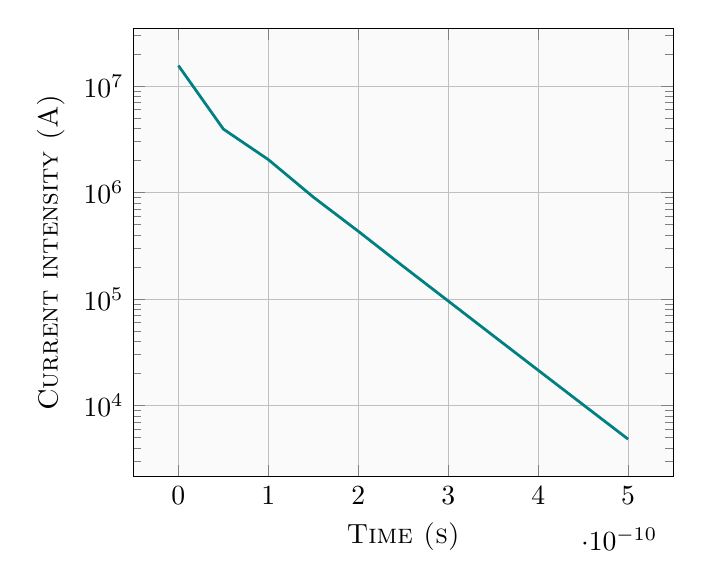
\begin{tikzpicture}[scale=1,>=latex]
\begin{axis}[ymode=log, xlabel=\textsc{{Time (s)}}, ylabel=\textsc{{Current intensity (A)}}, ymajorgrids, xmajorgrids, axis background/.style={fill=gray!4},, legend style={legend columns=2,at={(0.5,-0.2)},anchor=north}]
\addplot+[color=teal,line width=1pt,mark=none] coordinates {(0, 1.55782e+07) (5.0e-11, 3.94512e+06) (1e-10, 2.0403e+06) (1.5e-10, 906796) (2e-10 , 433197) (2.5e-10, 202728) (3e-10, 95922.9) (3.5e-10, 45317.9) (4e-10, 21472.3) (4.5e-10, 10183.3) (5e-10, 4836.51)};
\end{axis}
\end{tikzpicture}
\caption{$\eta_{\rm VV} = 10^4 ~\SI{}{\ohm\meter}$}
\label{fig:current_VVdiffusion_S2e-3_2e-5_time}
\end{subfigure}     
\caption{Evolution of the current intensity inside the vacuum vessel over time with two different vacuum vessel resistivities $\eta_{\rm VV}$ and a fixed resistivity elsewhere $\eta= 10^6 ~\SI{}{\ohm\meter}$}   
\end{figure}
\noindent With a resistivity value of $\eta_{\rm VV} = \SI{1e+4}{\ohm\meter}$ (i.e. a Lundquist number $S_{\rm VV} = \num{2.7646e-3}$) inside the vacuum vessel and $\eta = \SI{1e+6}{\ohm\meter}$ ($S = \num{2.7646e-5}$) elsewhere, we obtain the current evolution depicted in Figure~\ref{fig:current_VVdiffusion_S2e-3_2e-5_time}. 
The slope %at $t=0$ 
is now equal to:
\begin{equation}
a_2 := \dfrac{\ln(10^5) - \ln(10^6)}{\num{3e-10} - \num{1.5e-10}} = -\num{1.53e+10}.
\end{equation}

\noindent The characteristic $L/R$ or wall time is expressed as
\begin{equation}
\tau_{VV} = \dfrac{L}{R_t},
\end{equation}
with $L$ the inductance and the toroidal resistance
\begin{equation}
R_t = \dfrac{2 \pi R \eta}{\mathcal{A}};
\end{equation}
$\mathcal{A}$ being the cross section.
The current decay is such that 
\begin{equation}
I(t) = I_0 \exp(-\dfrac{t}{\tau_{VV}}).
\end{equation}
With the slopes computed previously, we can deduce that the resistivity value corresponding to $\tau_{VV} = \SI{500}{\milli\second}$ is: 
\begin{equation}
\eta_{\rm VV} = \SI{1.30288e-6}{\ohm\meter} .
\label{eqn:VVresistivity}
\end{equation}
\noindent With such a resistivity ($S_{\rm VV} = 21219200$) inside the vacuum vessel and $\eta = \SI{1.30288e-3}{\ohm\meter}$ ($S = 21219.2$) elsewhere, we obtain the current evolution depicted in Figure~\ref{fig:current_VVdiffusion_S2e+7_2e+4_time}. 
The slope %at $t=0$ 
is equal to:
\begin{equation}
a_3 := \dfrac{\ln(3922.26) - \ln(860919)}{3.858030 - 1.157409} = -1.99633062361,
\end{equation} 
which is very close to the expected value $\dfrac{-1}{\tau_{VV}} = \dfrac{-1}{0.5} = -2$.
\begin{figure}[!h]
\centering
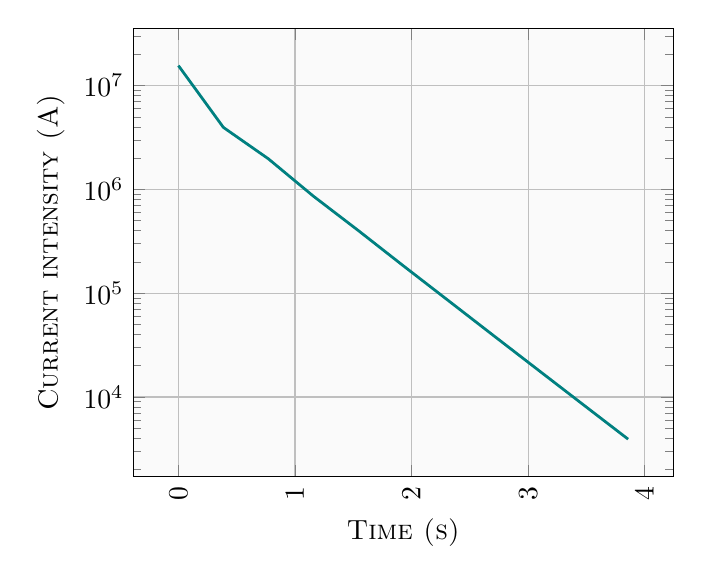
\begin{tikzpicture}[scale=1,>=latex]
\begin{axis}[ymode=log, xlabel=\textsc{{Time (s)}}, ylabel=\textsc{{Current intensity (A)}}, ymajorgrids, xmajorgrids, xticklabel style={rotate=90}, axis background/.style={fill=gray!4},, legend style={legend columns=2,at={(0.5,-0.2)},anchor=north}]
\addplot+[color=teal,line width=1pt,mark=none] coordinates {(0, 1.55781e+07) (0.3858, 3.95356e+06) (0.771606, 1.97043e+06) (1.157409, 860919) (1.543212 , 401278) (1.929015, 183727) (2.314818, 84977.2) (2.700621, 39265.7) (3.086424, 18195.9) (3.472227, 8441.54) (3.858030, 3922.26)};
\end{axis}
\end{tikzpicture}
\caption{Evolution of the current intensity inside the vacuum vessel over time with $\eta_{\rm VV} = \SI{1.30288e-6}{\ohm\meter}$}
\label{fig:current_VVdiffusion_S2e+7_2e+4_time}
\end{figure}

\subsection{Computing and refining the initial state for the quasi-static force-free model}

The quasi-static force-free model targets a post-thermal-quench plasma
in which the plasma beta, defined as the ratio of the plasma pressure
and the magnetic pressure, is negligibly small. We prepare such an
initial force-free state via a Grad-Shafranov
solve~\cite{Li-Tang2-SIAMJSC-2021} by zeroing out the plasma beta of
an original full-beta \SI{15}{\mega\ampere} ITER equilibrium, while holding the
poloidal magnetic flux fixed from the original full-beta \SI{15}{\mega\ampere}
free-boundary Grad-Shafranov equilibrium.  This frozen flux boundary
condition simply reflects the fact that on the time scale of the
thermal quench, which is anticipated to be on the order of a
millisecond and hence much shorter than the vacuum vessel wall time,
the vacuum vessel acts like a perfect flux conserver.  This initial
state thus has zero pressure gradient, \SI{15}{\mega\ampere} of toroidal plasma
current, and one x-point at the bottom. The details of the force-free
equilibrium solve can be found in Ref.~\cite{Li-Tang2-SIAMJSC-2021}.
The numerical solution, once transferred to the staggered grid of the
mimetic finite difference solver, has $(\nabla \times \B) \times \B$
that is not exactly zero but close to $10^{-3}$, and that introduces
an error at the first time step of the quasi-static model in
Equations~\eqref{eq:4.566} and~\eqref{eq:4.568} since the initial
velocity is nil. This gross violation of force-free condition creates
difficulties for the quasi-static force-free solver at the Newton
iteration of the first time step.

A workaround for this issue is to call a time-dependent model that
would decrease $(\nabla \times \B) \times \B$ and also compute a
velocity that would restore some balance in Equations~\eqref{eq:4.566}
and~\eqref{eq:4.568}.  This time-dependent model is as follows.
\begin{itemize}
\item In the plasma region:
\begin{align}
  \frac{\partial n_i}{\partial t} + \nabla\cdot\left(n_i{\V}_{i\perp}\right) = & ~0 \qquad \text{in} \quad  \Omega^{P}, \label{eq:4.596} \\
  m_i n_0 \frac{\partial {\V}_{i\perp} }{\partial t} - \nu m_i n_0 \nabla^2 \V_{i\perp} - \frac{1}{\mu_0} (\nabla\times{\B})\times{\B} = & ~0 \qquad \text{in} \quad \Omega^{P} , \label{eq:4.597} \\
  - \nabla^2 \Phi + \nabla\cdot\left[ {\V}_{i\perp}\times {\B}  \right] = & ~ 0 \qquad \text{in} \quad \Omega^{P}, \label{eq:4.598} \\
  \boldsymbol{\tau} - \nabla\Phi + {\V}_{i\perp}\times {\B}  = & ~ \mathbf{0} \qquad \text{in} \quad \Omega^{P}, \label{eq:4.599} \\
  \frac{\partial{\B}}{\partial t} + \nabla\times\boldsymbol{\tau} = & ~ \mathbf{0} \qquad \text{in} \quad \Omega^{P}. \label{eq:4.600}
\end{align}
\item In the wall region:
\begin{align}
\frac{\partial n_i}{\partial t} = & ~ 0 \qquad \text{in} \quad \Omega^{W}, \label{eq:4.601} \\
  {\V}_{i\perp} = & ~ \mathbf{0} \qquad \text{in} \quad \Omega^{W} , \label{eq:4.602} \\
  - \nabla^2 \Phi = & ~ 0 \qquad \text{in} \quad \Omega^{W} \label{eq:4.603} \\
  \boldsymbol{\tau} - \nabla\Phi = & ~ \mathbf{0} \qquad \text{in} \quad \Omega^{W}, \label{eq:4.604} \\
  \frac{\partial{\B}}{\partial t} + \nabla\times\boldsymbol{\tau} = & ~ \mathbf{0} \qquad \text{in} \quad \Omega^{W} . \label{eq:4.605}
\end{align}
\item At the wall/plasma interface:
\begin{align}
  {\V}_{i\perp} = ~ 0 \qquad \text{in} \quad \Gamma^{PW} , \label{eq:4.606} \\
  {\B} \cdot \mathbf{n} \qquad \text{continous across} \quad \Gamma^{PW} , \label{eq:4.607} \\
  \boldsymbol{\tau} \times \mathbf{n} \qquad \text{continous across} \quad \Gamma^{PW}. \label{eq:4.608}
\end{align}
\item At the outer rectangular boundary:
\begin{align}
  \Phi = & ~ \mathbf{0} \qquad \text{on} \quad \partial \Omega. \label{eq:4.609}
\end{align}
\end{itemize}
The resulting velocity $\V_{i\perp,0}$ and magnetic field $\B_0$ from
this time-dependent model %, which is run for about 2000 Alfven times
are then used to update $\boldsymbol{\tau}_0$ the divergence-free
component of the electric field and $\Phi_0$ the electrostatic
potential such that we have
\begin{itemize}
\item in the plasma region:
\begin{align}
  - \nabla^2 \Phi_0 - \nabla\cdot\left[ - {\V}_{i\perp,0}\times {\B_0} + \frac{\eta}{\mu_0}\left(\nabla\times{\B_0}\right) \right] = & ~ 0 \qquad \text{in} \quad \Omega^{P}, \label{eq:4.598_updatePh} \\
  \boldsymbol{\tau}_0 - \nabla\Phi_0 + {\V}_{i\perp,0}\times {\B_0} - \frac{\eta}{\mu_0}\left(\nabla\times{\B_0}\right) = & ~ \mathbf{0} \qquad \text{in} \quad \Omega^{P}, \label{eq:4.599_updatetau} 
\end{align}
\item in the wall region:
\begin{align}
  - \nabla^2 \Phi_0 - \nabla\cdot\left[ \frac{\eta}{\mu_0}\left(\nabla\times{\B_0}\right) \right] = & ~ 0 \qquad \text{in} \quad \Omega^{W} \label{eq:4.603_updatePhi} \\
  \boldsymbol{\tau}_0 - \nabla\Phi_0 - \frac{\eta}{\mu_0}\left(\nabla\times{\B_0}\right) = & ~ \mathbf{0} \qquad \text{in} \quad \Omega^{W}, \label{eq:4.604_updatetau} 
\end{align}
\end{itemize}
Finally, we set $n_0 = \SI{1e+20}{\centi\meter}^{-3}$ and that completes
the initial state $(n_0, {\V}_{i\perp,0}, \Phi_0, \boldsymbol{\tau}_0,
{\B_0} )$ for the quasi-static model.
  
\subsection{Comparing the different regularizations}  \label{sec:regularization}

As noted in section~\ref{sec:regularization}, the quasi-static
force-free model requires regularization that invokes either a
fictitious drag coefficient $\epsilon$ or an artificial viscosity
$\nu.$ Since they enter directly into the force-balance equation that
would otherwise constrain the magnetic field to be force-free, we
anticipate their presence will modify the quasi-static dynamics but
the effect will diminish as $\epsilon$ or $\nu$ gets smaller. This is
a convergence issue of $\mathbf{B}(\mathbf{x},t)$ as a function of
decreasing $\epsilon$ and $\nu.$ It is important to note that with
smaller $\epsilon$ or $\nu,$ the regularization becomes weaker so the
numerical matrix inversion for the implicit solve of the quasi-static
model becomes more difficult computationally. So a practically useful
regulization scheme should produce strong convergence in
$\mathbf{B}(\mathbf{x},t)$ solution for modestly small $\epsilon$ or
$\nu.$ For this convergence check, we will gauge the quality of the
solution for $\mathbf{B}$ through two quantities.  The first is the
vertical position of the magnetic axis $Z_a$ as a function of time
during a VDE.  The second is the total toroidal plasma current in the
chamber, $I_p(t),$ as a function of time during a VDE. Next we first
explain the set up of the test case, and then show how $Z_a(t)$ and
$I_p(t)$ scale with $\epsilon$ and $\nu.$

\begin{comment}
\subsection{Lundquist number $S = 2.7* 10^7$}
\end{comment}
We consider a 5-layer configuration for the resistivity as shown in
Figure~\ref{fig:5layer} with the following resistivity values:
\begin{itemize}
    \item $\eta = \SI{9.66e-6}{\ohm\meter}$ in the plasma chamber
      corresponding to values 1 and 2 for the levelset function in
      Figure~\ref{fig:5layer};
%    \item $\eta = 10^{-5}$ in the outer area of the plasma chamber located between the separatrix and the wall. This region corresponds to a value of 2 for the levelset function in Figure~\ref{fig:4layer}.     
    \item $\eta = \SI{4.4e-2}{\ohm\meter}$ in the rigid wall region
      corresponding to a value of 0 for the levelset function in
      Figure~\ref{fig:5layer};
    \item $\eta = \SI{1.30288e-6}{\ohm\meter}$ in the vacuum vessel
      corresponding to a value of -1 for the levelset function in
      Figure~\ref{fig:5layer};
    \item $\eta = \SI{1.30288e-3}{\ohm\meter}$ in the region
      outside the wall corresponding to a value of -2 for the levelset
      function in Figure~\ref{fig:5layer}.
\end{itemize}
and compare the results of the quasi-static models with fictitious
drag term~\eqref{eq:drag-regularize} and with fictitious viscous
term~\eqref{eq:viscous-regularize} using different viscosity and drag
coefficients. We plot the evolution in time of the z coordinate of the
magnetic axis and the current intensity in
Figures~\ref{fig:z_magneticaxis_15_15eV_time}
and~\ref{fig:current_time}. Note that after normalization of
Equation~\eqref{eq:viscous-regularize}, $\mu_0 \nu$ gets replaced by
the viscosity coefficient $\frac{1}{Re}$.

\begin{figure}[!h]
\centering
\begin{subfigure}[b]{0.47\textwidth} 
\centering
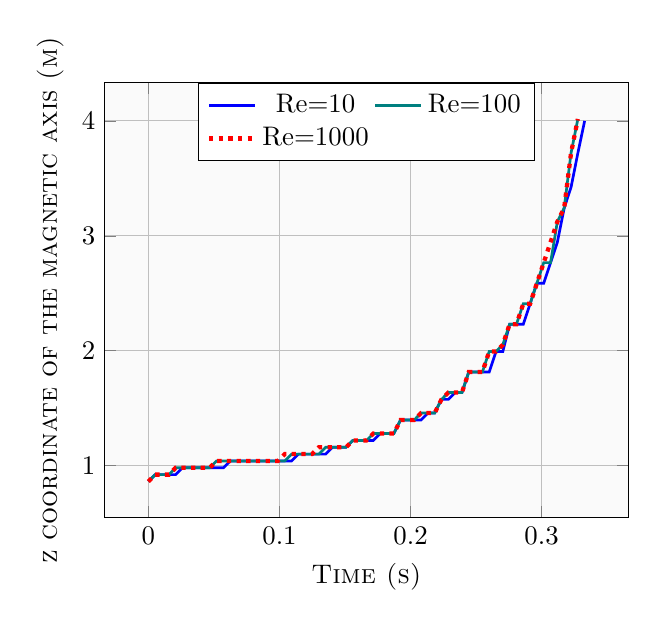
\begin{tikzpicture}[scale=0.97,>=latex]
\begin{axis}[xlabel=\textsc{{Time (s)}}, ylabel=\textsc{{z coordinate of the magnetic axis (m)}}, ymajorgrids, xmajorgrids, axis background/.style={fill=gray!4}, legend style={legend columns=2,at={(0.5,1.0)},anchor=north}]
\addplot+[color=blue,line width=1pt,mark=none] coordinates {(0, 0.86275)	(0.0052, 0.92225)	(0.0104, 0.92225)	(0.0156, 0.92225)	(0.0208, 0.92225)	(0.026, 0.98175)	(0.0312, 0.98175)	(0.0364, 0.98175)	(0.0416, 0.98175)	(0.0468, 0.98175)	(0.052, 0.98175)	(0.0572, 0.98175)	(0.0624, 1.04125)	(0.0676, 1.04125)	(0.0728, 1.04125)	(0.078, 1.04125)	(0.0832, 1.04125)	(0.0884, 1.04125)	(0.0936, 1.04125)	(0.0988, 1.04125)	(0.104, 1.04125)	(0.1092, 1.04125)	(0.1144, 1.10075)	(0.1196, 1.10075)	(0.1248, 1.10075)	(0.13, 1.10075)	         (0.1352, 1.10075)	(0.1404, 1.16025)	(0.1456, 1.16025)	(0.1508, 1.16025)	(0.156, 1.21975)	(0.1612, 1.21975)	(0.1664, 1.21975)	(0.1716, 1.21975)	(0.1768, 1.27925)	(0.182, 1.27925)	(0.1872, 1.27925)	(0.1924, 1.39825)	(0.1976, 1.39825)	(0.2028, 1.39825)	(0.208, 1.39825)	(0.2132, 1.45775)	(0.2184, 1.45775)	(0.2236, 1.57675)	(0.2288, 1.57675)   (0.234, 1.63625)	(0.2392, 1.63625)	(0.2444, 1.81475)	(0.2496, 1.81475)	(0.2548, 1.81475)	(0.26, 1.81475)   (0.2652, 1.99325)     (0.2704, 1.99325)     (0.2756, 2.23125)     (0.2808, 2.23125)     (0.286, 2.23125)       (0.2912, 2.40975)   (0.2964, 2.58825)     (0.3016, 2.58825)     (0.3068, 2.76675)     (0.3120, 2.94525)     (0.3172, 3.24275)     (0.3224, 3.42125)   (0.3276, 3.71875)   (0.3328, 4)};
\addplot+[color=teal,line width=1pt,mark=none] coordinates {(0, 0.86275)	(0.0052, 0.92225)	(0.0104, 0.92225)	(0.0156, 0.92225)	(0.0208, 0.98175)	(0.026, 0.98175)	(0.0312, 0.98175)	(0.0364, 0.98175)	(0.0416, 0.98175)	(0.0468, 0.98175)	(0.052, 1.04125)	(0.0572, 1.04125)	(0.0624, 1.04125)	(0.0676, 1.04125)	(0.0728, 1.04125)	(0.078, 1.04125)	(0.0832, 1.04125)	(0.0884, 1.04125)	(0.0936, 1.04125)	(0.0988, 1.04125)	(0.104, 1.04125)	(0.1092, 1.10075)	(0.1144, 1.10075)	(0.1196, 1.10075)	(0.1248, 1.10075)	(0.13, 1.10075)	         (0.1352, 1.16025)	(0.1404, 1.16025)	(0.1456, 1.16025)	(0.1508, 1.16025)	(0.156, 1.21975)	(0.1612, 1.21975)	(0.1664, 1.21975)	(0.1716, 1.27925)	(0.1768, 1.27925)	(0.182, 1.27925)	(0.1872, 1.27925)	(0.1924, 1.39825)	(0.1976, 1.39825)	(0.2028, 1.39825)	(0.208, 1.45775)	(0.2132, 1.45775)	(0.2184, 1.45775)	(0.2236, 1.57675)	(0.2288, 1.63625)   (0.234, 1.63625)	(0.2392, 1.63625)	(0.2444, 1.81475)	(0.2496, 1.81475)	(0.2548, 1.81475)	(0.26, 1.99325)   (0.2652, 1.99325)     (0.2704, 2.05275)     (0.2756, 2.23125)     (0.2808, 2.23125)     (0.286, 2.40975)       (0.2912, 2.40975)   (0.2964, 2.58825)     (0.3016, 2.76675)     (0.3068, 2.76675)     (0.3120, 3.12375)     (0.3172, 3.24275)     (0.3224, 3.71875)   (0.3276, 4.01625)};
\addplot+[color=red,line width=1pt,mark=none,ultra thick,dotted] coordinates {(0, 0.86275)	   (0.0052, 0.92225)	(0.0104, 0.92225)	(0.0156, 0.92225)	(0.0208, 0.98175)	(0.026, 0.98175)	(0.0312, 0.98175)	(0.0364, 0.98175)	(0.0416, 0.98175)	(0.0468, 0.98175)	(0.052, 1.04125)	(0.0572, 1.04125)	(0.0624, 1.04125)	(0.0676, 1.04125)	(0.0728, 1.04125)	(0.078, 1.04125)	(0.0832, 1.04125)	(0.0884, 1.04125)	(0.0936, 1.04125)	(0.0988, 1.04125)	(0.104, 1.10075)	(0.1092, 1.10075)	(0.1144, 1.10075)	(0.1196, 1.10075)	(0.1248, 1.10075)	(0.13, 1.16025)	         (0.1352, 1.16025)	(0.1404, 1.16025)	(0.1456, 1.16025)	(0.1508, 1.16025)	(0.156, 1.21975)	(0.1612, 1.21975)	(0.1664, 1.21975)	(0.1716, 1.27925)	(0.1768, 1.27925)	(0.182, 1.27925)	(0.1872, 1.27925)	(0.1924, 1.39825)	(0.1976, 1.39825)	(0.2028, 1.39825)	(0.208, 1.45775)	(0.2132, 1.45775)	(0.2184, 1.45775)	(0.2236, 1.57675)	(0.2288, 1.63625)   (0.234, 1.63625)	(0.2392, 1.63625)	(0.2444, 1.81475)	(0.2496, 1.81475)	(0.2548, 1.81475)	(0.26, 1.99325)   (0.2652, 1.99325)     (0.2704, 2.05275)     (0.2756, 2.23125)     (0.2808, 2.23125)     (0.286, 2.40975)       (0.2912, 2.40975)   (0.2964, 2.58825)     (0.3016, 2.76675)     (0.3068, 2.94525)     (0.3120, 3.12375)     (0.3172, 3.24275)     (0.3224, 3.71875)   (0.3276, 4.01625)};
\legend{Re=10,Re=100,Re=1000}
\end{axis}
\end{tikzpicture}
\caption{3 viscosity coefficients}
\label{fig:z_magneticaxis_15_15eV_time_Re1-100}
\end{subfigure} %
~
\begin{subfigure}[b]{0.47\textwidth}
\centering
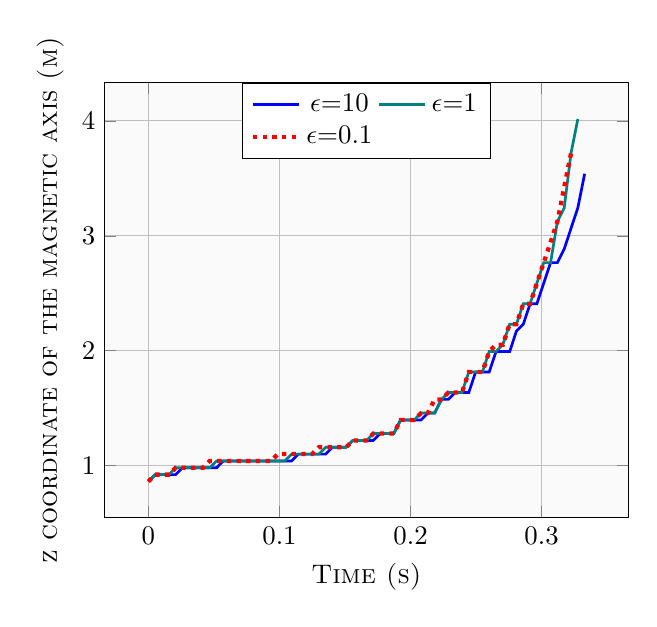
\begin{tikzpicture}[scale=0.97,>=latex]
\begin{axis}[xlabel=\textsc{{Time (s)}}, ylabel=\textsc{{z coordinate of the magnetic axis (m)}}, ymajorgrids, xmajorgrids, axis background/.style={fill=gray!4}, legend style={legend columns=2,at={(0.5,1.0)},anchor=north}]
\addplot+[color=blue,line width=1pt,mark=none] coordinates {(0, 0.86275)	(0.0052, 0.92225)	(0.0104, 0.92225)	(0.0156, 0.92225)	(0.0208, 0.92225)	(0.026, 0.98175)	(0.0312, 0.98175)	(0.0364, 0.98175)	(0.0416, 0.98175)	(0.0468, 0.98175)	(0.052, 0.98175)	(0.0572, 1.04125)	(0.0624, 1.04125)	(0.0676, 1.04125)	(0.0728, 1.04125)	(0.078, 1.04125)	(0.0832, 1.04125)	(0.0884, 1.04125)	(0.0936, 1.04125)	(0.0988, 1.04125)	(0.104, 1.04125)	(0.1092, 1.04125)	(0.1144, 1.10075)	(0.1196, 1.10075)	(0.1248, 1.10075)	(0.13, 1.10075)	         (0.1352, 1.10075)	(0.1404, 1.16025)	(0.1456, 1.16025)	(0.1508, 1.16025)	(0.156, 1.21975)	(0.1612, 1.21975)	(0.1664, 1.21975)	(0.1716, 1.21975)	(0.1768, 1.27925)	(0.182, 1.27925)	(0.1872, 1.27925)	(0.1924, 1.39825)	(0.1976, 1.39825)	(0.2028, 1.39825)	(0.208, 1.39825)	(0.2132, 1.45775)	(0.2184, 1.45775)	(0.2236, 1.57675)	(0.2288, 1.57675)    (0.234, 1.63625)	(0.2392, 1.63625)	(0.2444, 1.63625)      (0.2496, 1.81475)	(0.2548, 1.81475)	(0.26, 1.81475)	       (0.2652, 1.99325)	(0.2704, 1.99325)	(0.2756, 1.99325)      (0.2808, 2.17175)    (0.2860, 2.23125)      (0.2912, 2.40975)   (0.2964, 2.40975)   (0.3016, 2.58825)     (0.3068, 2.76675)     (0.3120, 2.76675)     (0.3172, 2.88575)      (0.3224, 3.06425)   (0.3276, 3.24275)   (0.3328, 3.54025)};
\addplot+[color=teal,line width=1pt,mark=none] coordinates {(0, 0.86275)	(0.0052, 0.92225)	(0.0104, 0.92225)	(0.0156, 0.92225)	(0.0208, 0.98175)	(0.026, 0.98175)	(0.0312, 0.98175)	(0.0364, 0.98175)	(0.0416, 0.98175)	(0.0468, 0.98175)	(0.052, 1.04125)	(0.0572, 1.04125)	(0.0624, 1.04125)	(0.0676, 1.04125)	(0.0728, 1.04125)	(0.078, 1.04125)	(0.0832, 1.04125)	(0.0884, 1.04125)	(0.0936, 1.04125)	(0.0988, 1.04125)	(0.104, 1.04125)	(0.1092, 1.10075)	(0.1144, 1.10075)	(0.1196, 1.10075)	(0.1248, 1.10075)	(0.13, 1.10075)	(0.1352, 1.16025)	(0.1404, 1.16025)	(0.1456, 1.16025)	(0.1508, 1.16025)	(0.156, 1.21975)	(0.1612, 1.21975)	(0.1664, 1.21975)	(0.1716, 1.27925)	(0.1768, 1.27925)	(0.182, 1.27925)	(0.1872, 1.27925)	(0.1924, 1.39825)	(0.1976, 1.39825)	(0.2028, 1.39825)	(0.208, 1.45775)	(0.2132, 1.45775)	(0.2184, 1.45775)	(0.2236, 1.57675)	(0.2288, 1.63625)   (0.234, 1.63625)	(0.2392, 1.63625)	(0.2444, 1.81475)	(0.2496, 1.81475)	(0.2548, 1.81475)	(0.26, 1.99325)   (0.2652, 1.99325)     (0.2704, 2.05275)     (0.2756, 2.23125)     (0.2808, 2.23125)     (0.286, 2.40975)      (0.2912, 2.40975)   (0.2964, 2.58825)     (0.3016, 2.76675)     (0.3068, 2.76675)     (0.3120, 3.12375)     (0.3172, 3.24275)    (0.3224, 3.71875)  (0.3276, 4.01625)};
%last two are already set
\addplot+[color=red,line width=1pt,mark=none,ultra thick,dotted] coordinates {(0, 0.86275)	(0.0052, 0.92225)	(0.0104, 0.92225)	(0.0156, 0.92225)	(0.0208, 0.98175)	(0.026, 0.98175)	(0.0312, 0.98175)	(0.0364, 0.98175)	(0.0416, 0.98175)	(0.0468, 1.04125)	(0.052, 1.04125)	(0.0572, 1.04125)	(0.0624, 1.04125)	(0.0676, 1.04125)	(0.0728, 1.04125)	(0.078, 1.04125)	(0.0832, 1.04125)	(0.0884, 1.04125)	(0.0936, 1.04125)	(0.0988, 1.10075)	(0.104, 1.10075)	(0.1092, 1.10075)	(0.1144, 1.10075)	(0.1196, 1.10075)	(0.1248, 1.10075)	(0.13, 1.16025)	(0.1352, 1.16025)	(0.1404, 1.16025)	(0.1456, 1.16025)	(0.1508, 1.16025)	(0.156, 1.21975)	(0.1612, 1.21975)	(0.1664, 1.21975)	(0.1716, 1.27925)	(0.1768, 1.27925)	(0.182, 1.27925)	(0.1872, 1.27925)	(0.1924, 1.39825)	(0.1976, 1.39825)	(0.2028, 1.39825)	(0.208, 1.45775)	(0.2132, 1.45775)	(0.2184, 1.57675)	(0.2236, 1.57675)	(0.2288, 1.63625)   (0.234, 1.63625)	(0.2392, 1.63625)	(0.2444, 1.81475)	(0.2496, 1.81475)	(0.2548, 1.81475)	(0.26, 1.99325)   (0.2652, 2.05275)     (0.2704, 2.05275)     (0.2756, 2.23125)     (0.2808, 2.23125)     (0.286, 2.40975)      (0.2912, 2.40975)   (0.2964, 2.58825)     (0.3016, 2.76675)     (0.3068, 2.94525)     (0.3120, 3.12375)     (0.3172, 3.42125)     (0.3224, 3.71875) };
\legend{$\epsilon$=10,$\epsilon$=1,$\epsilon$=0.1}
\end{axis}
\end{tikzpicture}
\caption{3 drag coefficients}
\label{fig:z_magneticaxis_15_15eV_time_eps+1-1}
\end{subfigure} 
\caption{Evolution of the z coordinate of the magnetic axis over time for different viscosity and drag coefficients}
\label{fig:z_magneticaxis_15_15eV_time}
\end{figure}

\begin{figure}[!h]
\centering
\begin{subfigure}[b]{0.47\textwidth} 
\centering
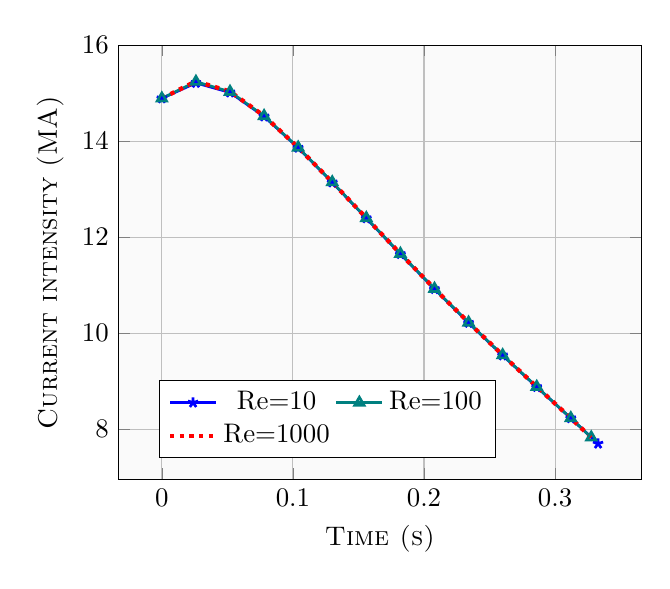
\begin{tikzpicture}[scale=0.97,>=latex]
\begin{axis}[scaled y ticks=base 10:-6, ytick scale label code/.code={}, xlabel=\textsc{{Time (s)}}, ylabel=\textsc{{Current intensity (MA)}}, ymajorgrids, xmajorgrids, axis background/.style={fill=gray!4}, legend style={legend columns=2,at={(0.4,0.05)},anchor=south}]
\addplot+[color=blue,line width=1pt,mark=star] coordinates {(0, 1.48934e+07) (0.026, 1.52149e+07) (0.052, 1.50161e+07) (0.078, 1.45168e+07) (0.104 , 1.38643e+07) (0.13, 1.31421e+07) (0.156, 1.23954e+07) (0.182, 1.16501e+07) (0.208, 1.09213e+07) (0.234, 1.02167e+07) (0.26, 9.53784e+06) (0.286, 8.87986e+06) (0.312, 8.22953e+06) (0.3328, 7.69845e+06)};
\addplot+[color=teal,line width=1pt,mark=triangle] coordinates {(0, 1.48934e+07) (0.026, 1.52405e+07) (0.052, 1.5032e+07) (0.078, 1.45262e+07) (0.104 , 1.38697e+07) (0.13, 1.31466e+07) (0.156, 1.24002e+07) (0.182, 1.16557e+07) (0.208, 1.09273e+07) (0.234, 1.02225e+07) (0.26, 9.54294e+06) (0.286, 8.88372e+06) (0.312, 8.23127e+06) (0.3276, 7.82844e+06)};
\addplot+[color=red,line width=1pt,mark=none,ultra thick,dotted] coordinates {(0, 1.48934e+07) (0.026, 1.52495e+07) (0.052, 1.50363e+07) (0.078, 1.45283e+07) (0.104 , 1.38704e+07) (0.13, 1.31472e+07) (0.156, 1.24011e+07) (0.182, 1.16571e+07) (0.208, 1.09291e+07) (0.234, 1.02241e+07) (0.26, 9.54422e+06) (0.286, 8.88477e+06) (0.312, 8.23172e+06) (0.3276, 7.82664e+06)};
\legend{Re=10,Re=100,Re=1000}
\end{axis}
\end{tikzpicture}
\caption{3 viscosity coefficients}
\label{fig:current_variousvisc_time}
\end{subfigure}%
~
\begin{subfigure}[b]{0.47\textwidth} 
\centering
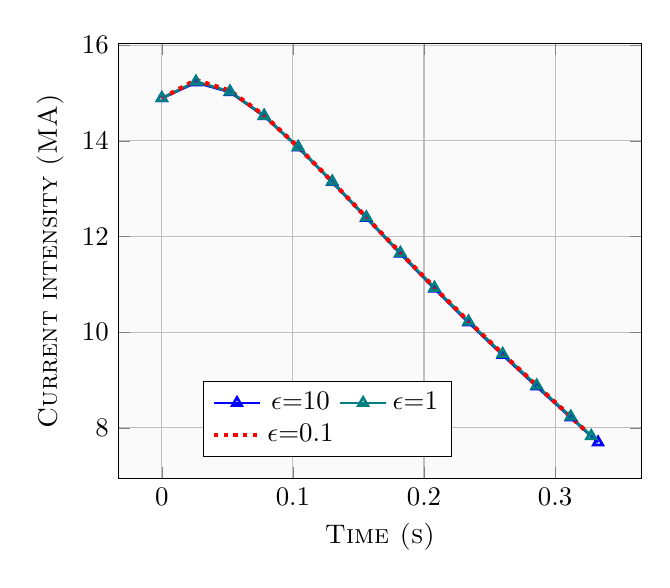
\begin{tikzpicture}[scale=0.97,>=latex]
\begin{axis}[scaled y ticks=base 10:-6, ytick scale label code/.code={}, xlabel=\textsc{{Time (s)}}, ylabel=\textsc{{Current intensity (MA)}}, ymajorgrids, xmajorgrids, axis background/.style={fill=gray!4}, legend style={legend columns=2,at={(0.4,0.05)},anchor=south}]
\addplot+[color=blue,line width=1pt,mark=triangle] coordinates {(0, 1.48934e+07) (0.026, 1.5222e+07) (0.052, 1.50214e+07) (0.078, 1.45207e+07) (0.104 , 1.38657e+07) (0.13, 1.3141e+07) (0.156, 1.23914e+07) (0.182, 1.16431e+07) (0.208, 1.09114e+07) (0.234, 1.0204e+07) (0.26, 9.52287e+06) (0.286, 8.86403e+06) (0.312, 8.21639e+06) (0.3328, 7.69489e+06)};
\addplot+[color=teal,line width=1pt,mark=triangle] coordinates {(0, 1.48934e+07) (0.026, 1.52405e+07) (0.052, 1.5032e+07) (0.078, 1.45262e+07) (0.104 , 1.38697e+07) (0.13, 1.31466e+07) (0.156, 1.24002e+07) (0.182, 1.16557e+07) (0.208, 1.09273e+07) (0.234, 1.02225e+07) (0.26, 9.54294e+06) (0.286, 8.88372e+06) (0.312, 8.23127e+06)  (0.3276, 7.82844e+06)};
\addplot+[color=red,line width=1pt,mark=none,ultra thick,dotted] coordinates {(0, 1.48934e+07) (0.026, 1.52739e+07) (0.052, 1.50496e+07) (0.078, 1.45334e+07) (0.104 , 1.38713e+07) (0.13, 1.31469e+07) (0.156, 1.24011e+07) (0.182, 1.16581e+07) (0.208, 1.09313e+07) (0.234, 1.02267e+07) (0.26, 9.5458e+06) (0.286, 8.88566e+06) (0.312, 8.22992e+06) (0.3224, 7.95837e+06)};
\legend{$\epsilon$=10,$\epsilon$=1,$\epsilon$=0.1}
\end{axis}
\end{tikzpicture}
\caption{3 drag coefficients}
\label{fig:current_variousdrag_time}
\end{subfigure}
\caption{Evolution of the current intensity inside the plasma chamber over time with different fictitious viscosity and drag coefficients}
\label{fig:current_time}
\end{figure}

\noindent We observe in Figures~\ref{fig:z_magneticaxis_15_15eV_time}
and~\ref{fig:current_time} that there is no significant change in the
curves for the current intensity and magnetic axis coordinate when we
vary the fictitious viscosity/drag coefficients, which could indicate
that the regularized model has already converged with such values and
there is no need to further decrease the regularization term as that
would induce more computational effort for the solver but with little
and insignificant impact on the relevant physical indicators or
properties.

% VDE happens at timestep 62 for drag coefficient epsilon = 0.1
% VDE happens at timestep 63 for drag coefficient epsilon = 1
% VDE happens at timestep 64 for drag coefficient epsilon = 10
% VDE happens at timestep 64 for drag coefficient Re = 10
% VDE happens at timestep 63 for drag coefficient Re = 100
% VDE happens at timestep 63 for drag coefficient Re = 1000

\noindent A subtler effect of regularization, as explained in
section~\ref{sec:regularization}, is that it sets a radial electric
field $\phi(\psi),$ which is not constrained by the quasi-static
force-free model. This is thus an artificial radial electric field,
which interestingly enough, does not modify the magnetic field
evolution directly, since the curl of an electrostatic field vanishes
in the Faraday's law.  In Fig.~\ref{fig:EP_avg_psi_isovolumes}, we numerically compute
$\phi(\psi)$ from $\Phi(R,Z)$ by performing an average of $\Phi$ along
the field lines which are contours of poloidal magnetic flux $\psi.$
This $\phi(\Psi)$ is then plotted as a function of $\psi.$ Here we
shall classify two classes of magnetic field lines or constant $\psi$
surfaces (contour lines in the poloidal cross section of an
axisymmetric configuration).  Where $\psi$ forms closed contours in
the plasma domain, one has closed flux surfaces.  There are regions in
which $\psi$ contours or magnetic field lines intercept the chamber
wall, these are known as the open flux or magnetic field line region.
Since the chamber wall is a conductor and $\Phi$ is set to zero there,
so $\phi$ on the open flux region is close to zero, in the order of
$10^{-10}$ to $10^{-8}$ (normalized unit) range.  The radial
electrostatic potential $\phi(\psi)$ can take on a much larger value
inside the closed flux region, resulting in a sizable radial electric
field across the separatrix (if it exists) or the last closed flux
surface that scrapes off the chamber wall.

\noindent By comparing Fig.~\ref{fig:EP_avg_psi_isovolumes_visc} and
Fig.~\ref{fig:EP_avg_psi_isovolumes_drag}, one can see that both the
fictitious drag $(\epsilon)$ and artificial viscosity $(\nu)$ produce
$\phi(\psi)$ of comparable amplitude. In the case of artificial
viscosity, the $Re=100$ and $Re=1000$ cases appear to converge to the
same $\phi(\psi).$ The fictitious drag coefficients of $\epsilon=10$
and $\epsilon=0.1$ evidently yield $\phi(\psi)$ with sizable
difference in the closed flux region. It should be emphasized again
that the $\phi(\psi)$ so produced is an artificial radial electric
field, entirely the result of the regularization scheme. The
quasi-static MHD model itself does not physically constrain
$\phi(\psi).$

\noindent At a later time, all the fictitious drag and artificial viscosity coefficients produce almost identical $\phi(\psi)$ amplitudes. This could be observed in  Figure~\ref{fig:EP_avg_psi_isovolumes_50dt} that shows the curves of electrostatic potential average in function of the poloidal magnetic flux function after 50 time steps, which corresponds to the time when the magnetic axis moves to mid-way (in vertical position) between the eventual impact point at the first wall and the initial state.


\pgfplotstableread{data_to_plot/dataRe10.txt}\tableone
\pgfplotstablecreatecol[create col/expr={-log10(-\thisrow{y} * 55000000)}]{log}\tableone
\pgfplotstablecreatecol[create col/expr={5*(\thisrow{x})}]{nonnormx}\tableone


\pgfplotstableread{data_to_plot/dataRe100.txt}\tabletwo
\pgfplotstablecreatecol[create col/expr={-log10(-\thisrow{y} * 55000000)}]{log}\tabletwo
\pgfplotstablecreatecol[create col/expr={5*(\thisrow{x})}]{nonnormx}\tabletwo


\pgfplotstableread{data_to_plot/dataRe1000.txt}\tablethree
\pgfplotstablecreatecol[create col/expr={-log10(-\thisrow{y} * 55000000)}]{log}\tablethree
\pgfplotstablecreatecol[create col/expr={5*(\thisrow{x})}]{nonnormx}\tablethree

\pgfplotstableread{data_to_plot/datadampV+1.txt}\tablefour
\pgfplotstablecreatecol[create col/expr={1/log10(-\thisrow{y})}]{log}\tablefour
\pgfplotstablecreatecol[create col/expr={5*(\thisrow{x})}]{nonnormx}\tablefour


\pgfplotstableread{data_to_plot/datadampV-1.txt}\tablesix
%\pgfplotstablecreatecol[create col/expr={-log10(-\thisrow{y}) * (\thisrow{y}<0) + log10(\thisrow{y}) * (\thisrow{y}>0)}]{log}\tablefive
\pgfplotstablecreatecol[create col/expr={\thisrow{y} > 0 ? -1/log10(\thisrow{y}) : 1/log10(-\thisrow{y})}]{log}\tablesix 
\pgfplotstablecreatecol[create col/expr={5*(\thisrow{x})}]{nonnormx}\tablesix

\pgfplotstableread{data_to_plot/datadampV0.txt}\tablefive
\pgfplotstablecreatecol[create col/expr={\thisrow{y} > 0 ? -1/log10(\thisrow{y}) : 1/log10(-\thisrow{y})}]{log}\tablefive 
\pgfplotstablecreatecol[create col/expr={5*(\thisrow{x})}]{nonnormx}\tablefive


\pgfplotstableread{data_to_plot/datadampV-2.txt}\tablesixbis
%\pgfplotstablecreatecol[create col/expr={-log10(-\thisrow{y}) * (\thisrow{y}<0) + log10(\thisrow{y}) * (\thisrow{y}>0)}]{log}\tablefive
\pgfplotstablecreatecol[create col/expr={\thisrow{y} > 0 ? -1/log10(\thisrow{y}) : 1/log10(-\thisrow{y})}]{log}\tablesixbis 
\pgfplotstablecreatecol[create col/expr={5*(\thisrow{x})}]{nonnormx}\tablesixbis

\begin{figure}[!h]
\centering
\begin{subfigure}[b]{0.47\textwidth} 
\begin{tikzpicture}[scale=0.90,>=latex]
\begin{axis}[xlabel=\textsc{{Poloidal magnetic flux function}}, ylabel=\textsc{{Electrostatic potential average}} , ytick={4,3,2,1,0,-1,-2}, yticklabels={$-10^{-4}$,$-10^{-3}$,$-10^{-2}$,$-10^{-1}$,$-1$,$-10$,$-100$}, ymajorgrids, xmajorgrids, axis background/.style={fill=gray!4}, legend style={legend columns=2,at={(0.66,1)},anchor=north}]
%\addplot+[color=blue,line width=1pt,mark=star] coordinates {(-8.29942, 1.48934e+07) (-7.16289, 1.52495e+07) (-6.01974, 1.50363e+07) (-4.87658, 1.45283e+07) (-3.73343 , 1.38704e+07) (-2.59028, 1.31472e+07) (-1.44713, 1.24011e+07) (-0.303973, 1.16571e+07) (0.83918, 1.09291e+07) (1.88233, 1.02241e+07) };
%\addplot+[color=teal,line width=1pt,mark=triangle] coordinates {(-8.29942, -1.8950599e-11) (-7.16289, -8.2132436e-11) (-6.01974, -2.3033332e-10) (-4.87658, -1.20993374e-9) (-3.73343 , -2.21793749e-9) (-2.59028, -1.93624069e-8) (-1.44713, -0.00000407647) (-0.303973, -0.00000387466) (0.83918, -0.00000304414) (1.88233, -8.08733057e-7)};
%\addplot+[color=red,line width=1pt,mark=none,ultra thick,dotted] coordinates {(-8.29942, -1.4556861e-11) (-7.16289, -6.4457328e-11) (-6.01974, -2.0733733e-10) (-4.87658, -1.16348118e-9) (-3.73343 , -2.13538999e-9) (-2.59028, -1.69946902e-8) (-1.44713, -0.00000468606) (-0.303973, -0.00000393359) (0.83918, -0.00000300482) (1.88233, -8.46751698e-7)};
\addplot+[color=blue,line width=1pt,mark=star] table[x=nonnormx, y=log] \tableone;
\addplot+[color=teal,line width=1pt,mark=triangle] table[x=nonnormx, y=log] \tabletwo;
\addplot+[color=red,line width=1pt,mark=o] table[x=nonnormx, y=log] \tablethree;
\legend{Re=10,Re=100,Re=1000}
\end{axis}
\end{tikzpicture}
\caption{3 viscosity coefficients}
\label{fig:EP_avg_psi_isovolumes_visc}
\end{subfigure}%
~
\begin{subfigure}[b]{0.47\textwidth} 
\centering
\begin{tikzpicture}[scale=0.90,>=latex]
\begin{axis}[xlabel=\textsc{{Poloidal magnetic flux function}}, ylabel=\textsc{{Electrostatic potential average}} , ytick={-0.0833,-0.125,-0.1666,-0.25,0,0.1666,0.25}, yticklabels={$-10^{-4.26}$,$-10^{0.26}$,$-10^{1.74}$,$-10^{3.74}$,0,$10^{1.74}$,$10^{3.74}$}, ymajorgrids, xmajorgrids, axis background/.style={fill=gray!4}, legend style={legend columns=2,at={(0.5,1)},anchor=north}]
%ytick={-0.0833,-0.125,-0.1666,-0.25,0,0.1666,0.25}, yticklabels={$-10^{-12}$,$-10^{-8}$,$-10^{-6}$,$-10^{-4}$,0,$10^{-6}$,$10^{-4}$}, ymajorgrids, xmajorgrids, axis background/.style={fill=gray!4}, legend style={legend columns=2,at={(0.5,1)},anchor=north}]
%ytick={-0.1515,-0.227,-0.303,-0.4545,0,0.303,0.4545}, yticklabels={$-10^{-4}$,$-1$,$-10^{2}$,$-10^{4}$,$1$,$10^{2}$,$10^{4}$},
\addplot+[color=blue,line width=1pt,mark=star] table[x=nonnormx, y=log] \tablefour;
\addplot+[color=teal,line width=1pt,mark=triangle] table[x=nonnormx, y=log] \tablefive;
\addplot+[color=red,line width=1pt,mark=o] table[x=nonnormx, y=log] \tablesix;
\addplot+[color=black,line width=1pt,mark=none] table[x=nonnormx, y=log] \tablesixbis;
\legend{$\epsilon$=10,$\epsilon$=1,$\epsilon$=0.1,$\epsilon$=0.01}
\end{axis}
\end{tikzpicture}
\caption{4 drag coefficients}
\label{fig:EP_avg_psi_isovolumes_drag}
\end{subfigure}
\caption{Evolution of the electrostatic potential average over poloidal magnetic flux function with different fictitious viscosity and drag coefficients at the first time step}
\label{fig:EP_avg_psi_isovolumes}
\end{figure}


%Add electrostatic potential average plots at t = 25 dt, i.e. t = 0.13

\pgfplotstableread{data_to_plot/datadampV+1_25dt.txt}\tablethirteen
\pgfplotstablecreatecol[create col/expr={\thisrow{y} > 0 ? -1/log10(\thisrow{y}) : 1/log10(-\thisrow{y})}]{log}\tablethirteen
\pgfplotstablecreatecol[create col/expr={5*(\thisrow{x})}]{nonnormx}\tablethirteen


\pgfplotstableread{data_to_plot/datadampV0_25dt.txt}\tablefourteen
\pgfplotstablecreatecol[create col/expr={\thisrow{y} > 0 ? -1/log10(\thisrow{y}) : 1/log10(-\thisrow{y})}]{log}\tablefourteen
\pgfplotstablecreatecol[create col/expr={5*(\thisrow{x})}]{nonnormx}\tablefourteen


\pgfplotstableread{data_to_plot/datadampV-1_25dt.txt}\tablefifteen
\pgfplotstablecreatecol[create col/expr={\thisrow{y} > 0 ? -1/log10(\thisrow{y}) : 1/log10(-\thisrow{y})}]{log}\tablefifteen
\pgfplotstablecreatecol[create col/expr={5*(\thisrow{x})}]{nonnormx}\tablefifteen


\pgfplotstableread{data_to_plot/dataRe10_25dt.txt}\tablesixteen
\pgfplotstablecreatecol[create col/expr={\thisrow{y} > 0 ? -1/log10(\thisrow{y}) : 1/log10(-\thisrow{y})}]{log}\tablesixteen
\pgfplotstablecreatecol[create col/expr={5*(\thisrow{x})}]{nonnormx}\tablesixteen


\pgfplotstableread{data_to_plot/dataRe100_25dt.txt}\tableseventeen
\pgfplotstablecreatecol[create col/expr={\thisrow{y} > 0 ? -1/log10(\thisrow{y}) : 1/log10(-\thisrow{y})}]{log}\tableseventeen
\pgfplotstablecreatecol[create col/expr={5*(\thisrow{x})}]{nonnormx}\tableseventeen


\pgfplotstableread{data_to_plot/dataRe1000_25dt.txt}\tableeighteen
\pgfplotstablecreatecol[create col/expr={\thisrow{y} > 0 ? -1/log10(\thisrow{y}) : 1/log10(-\thisrow{y})}]{log}\tableeighteen
\pgfplotstablecreatecol[create col/expr={5*(\thisrow{x})}]{nonnormx}\tableeighteen


\begin{figure}[!h]
\centering
\begin{subfigure}[b]{0.47\textwidth} 
\begin{tikzpicture}[scale=0.90,>=latex]
\begin{axis}[xlabel=\textsc{{Poloidal magnetic flux function}}, ylabel=\textsc{{Electrostatic potential average}} , ytick={-0.1666,-0.13768,-0.10266,0,0.1687}, yticklabels={-55,-3,$-10^{-2}$,0,65}, ymajorgrids, xmajorgrids, axis background/.style={fill=gray!4}, legend style={legend columns=2,at={(0.4,1)},anchor=north}]
\addplot+[color=blue,line width=1pt,mark=star] table[x=nonnormx, y=log] \tablesixteen;
\addplot+[color=teal,line width=1pt,mark=triangle] table[x=nonnormx, y=log] \tableseventeen;
\addplot+[color=red,line width=1pt,mark=o] table[x=nonnormx, y=log] \tableeighteen;
\legend{Re=10,Re=100,Re=1000}
\end{axis}
\end{tikzpicture}
\caption{3 viscosity coefficients}
\label{fig:EP_avg_psi_isovolumes_visc_25dt}
\end{subfigure}%
~
\begin{subfigure}[b]{0.47\textwidth} 
\centering
\begin{tikzpicture}[scale=0.90,>=latex]
\begin{axis}[xlabel=\textsc{{Poloidal magnetic flux function}}, ylabel=\textsc{{Electrostatic potential average}} , ytick={-0.1666,-0.13768,-0.10266,0,0.1687}, yticklabels={-55,-3,$-10^{-2}$,0,65}, ymajorgrids, xmajorgrids, axis background/.style={fill=gray!4}, legend style={legend columns=2,at={(0.4,1)},anchor=north}]
% ytick={-0.1666,-0.14836,-0.13768,-0.10266,0,0.1687}, yticklabels={-55,-10,-3,$-10^{-2}$,0,65}
\addplot+[color=blue,line width=1pt,mark=star] table[x=nonnormx, y=log] \tablethirteen;
\addplot+[color=teal,line width=1pt,mark=triangle] table[x=nonnormx, y=log] \tablefourteen;
\addplot+[color=red,line width=1pt,mark=o] table[x=nonnormx, y=log] \tablefifteen;
\legend{$\epsilon$=10,$\epsilon$=1,$\epsilon$=0.1}
\end{axis}
\end{tikzpicture}
\caption{2 drag coefficients}
\label{fig:EP_avg_psi_isovolumes_drag_25dt}
\end{subfigure}
\caption{Evolution of the electrostatic potential average over poloidal magnetic flux function with different fictitious viscosity and drag coefficients after 25 time steps}
\label{fig:EP_avg_psi_isovolumes_25dt}
\end{figure}


%Add electrostatic potential average plots at t = 50 dt, i.e. t = 0.26

\pgfplotstableread{data_to_plot/datadampV+1_50dt.txt}\tableten
\pgfplotstablecreatecol[create col/expr={-log10(-\thisrow{y} * 55000000)}]{log}\tableten
\pgfplotstablecreatecol[create col/expr={5*(\thisrow{x})}]{nonnormx}\tableten


\pgfplotstableread{data_to_plot/datadampV0_50dt.txt}\tableeleven
\pgfplotstablecreatecol[create col/expr={-log10(-\thisrow{y} * 55000000)}]{log}\tableeleven
\pgfplotstablecreatecol[create col/expr={5*(\thisrow{x})}]{nonnormx}\tableeleven


\pgfplotstableread{data_to_plot/datadampV-1_50dt.txt}\tabletwelve
\pgfplotstablecreatecol[create col/expr={-log10(-\thisrow{y} * 55000000)}]{log}\tabletwelve
\pgfplotstablecreatecol[create col/expr={5*(\thisrow{x})}]{nonnormx}\tabletwelve


\pgfplotstableread{data_to_plot/dataRe10_50dt.txt}\tableseven
\pgfplotstablecreatecol[create col/expr={-log10(-\thisrow{y} * 55000000)}]{log}\tableseven
\pgfplotstablecreatecol[create col/expr={5*(\thisrow{x})}]{nonnormx}\tableseven


\pgfplotstableread{data_to_plot/dataRe100_50dt.txt}\tableeight
\pgfplotstablecreatecol[create col/expr={-log10(-\thisrow{y} * 55000000)}]{log}\tableeight
\pgfplotstablecreatecol[create col/expr={5*(\thisrow{x})}]{nonnormx}\tableeight


\pgfplotstableread{data_to_plot/dataRe1000_50dt.txt}\tablenine
\pgfplotstablecreatecol[create col/expr={-log10(-\thisrow{y} * 55000000)}]{log}\tablenine
\pgfplotstablecreatecol[create col/expr={5*(\thisrow{x})}]{nonnormx}\tablenine


\begin{figure}[!h]
\centering
\begin{subfigure}[b]{0.47\textwidth} 
\begin{tikzpicture}[scale=0.90,>=latex]
\begin{axis}[xlabel=\textsc{{Poloidal magnetic flux function}}, ylabel=\textsc{{Electrostatic potential average}} , ytick={4,3,2,1,0,-1,-2}, yticklabels={$-10^{-4}$,$-10^{-3}$,$-10^{-2}$,$-10^{-1}$,$-1$,$-10$,$-100$}, ymajorgrids, xmajorgrids, axis background/.style={fill=gray!4}, legend style={legend columns=2,at={(0.66,1)},anchor=north}]
\addplot+[color=blue,line width=1pt,mark=star] table[x=nonnormx, y=log] \tableseven;
\addplot+[color=teal,line width=1pt,mark=triangle] table[x=nonnormx, y=log] \tableeight;
\addplot+[color=red,line width=1pt,mark=o] table[x=nonnormx, y=log] \tablenine;
\legend{Re=10,Re=100,Re=1000}
\end{axis}
\end{tikzpicture}
\caption{3 viscosity coefficients}
\label{fig:EP_avg_psi_isovolumes_visc_50dt}
\end{subfigure}%
~
\begin{subfigure}[b]{0.47\textwidth} 
\centering
\begin{tikzpicture}[scale=0.90,>=latex]
\begin{axis}[xlabel=\textsc{{Poloidal magnetic flux function}}, ylabel=\textsc{{Electrostatic potential average}} , ytick={4,3,2,1,0,-1,-2}, yticklabels={$-10^{-4}$,$-10^{-3}$,$-10^{-2}$,$-10^{-1}$,$-1$,$-10$,$-100$}, ymajorgrids, xmajorgrids, axis background/.style={fill=gray!4}, legend style={legend columns=2,at={(0.6,1)},anchor=north}]
\addplot+[color=blue,line width=1pt,mark=star] table[x=nonnormx, y=log] \tableten;
\addplot+[color=teal,line width=1pt,mark=triangle] table[x=nonnormx, y=log] \tableeleven;
\addplot+[color=red,line width=1pt,mark=o] table[x=nonnormx, y=log] \tabletwelve;
\legend{$\epsilon$=10,$\epsilon$=1,$\epsilon$=0.1}
\end{axis}
\end{tikzpicture}
\caption{2 drag coefficients}
\label{fig:EP_avg_psi_isovolumes_drag_50dt}
\end{subfigure}
\caption{Evolution of the electrostatic potential average over poloidal magnetic flux function with different fictitious viscosity and drag coefficients after 50 time steps}
\label{fig:EP_avg_psi_isovolumes_50dt}
\end{figure}


\begin{figure}[!h]
\centering
\begin{subfigure}[b]{0.32\textwidth} 
\begin{center}
\includegraphics[width=\textwidth]{psi_Re10.png}
\caption{${\mathrm Re}=10$}
\label{fig:psi_drag_10}
\end{center}
\end{subfigure}%
~
\begin{subfigure}[b]{0.32\textwidth} 
\begin{center}
\includegraphics[width=\textwidth]{psi_Re100.png}
\caption{${\mathrm Re}=100$}
\label{fig:psi_drag_100}
\end{center}
\end{subfigure}%
~
\begin{subfigure}[b]{0.32\textwidth} 
\begin{center}
\includegraphics[width=\textwidth]{psi_Re1000.png}
\caption{${\mathrm Re}=1000$}
\label{fig:psi_drag_1000}
\end{center}
\end{subfigure}
\caption{The poloidal magnetic flux function with different fictitious viscosity coefficients at the first time step}
\label{fig:psi_1st_step}
\end{figure}

\begin{figure}[!h]
\centering
\begin{subfigure}[b]{0.32\textwidth} 
\begin{center}
\includegraphics[width=\textwidth]{EP_Re10.png}
\caption{${\mathrm Re}=10$}
\label{fig:EP_drag_10}
\end{center}
\end{subfigure}%
~
\begin{subfigure}[b]{0.32\textwidth} 
\begin{center}
\includegraphics[width=\textwidth]{EP_Re100.png}
\caption{${\mathrm Re}=100$}
\label{fig:EP_drag_100}
\end{center}
\end{subfigure}%
~
\begin{subfigure}[b]{0.32\textwidth} 
\begin{center}
\includegraphics[width=\textwidth]{EP_Re1000.png}
\caption{${\mathrm Re}=1000$}
\label{fig:EP_drag_1000}
\end{center}
\end{subfigure}
\caption{The electrostatic potential with different fictitious viscosity coefficients at the first time step}
\label{fig:EP_1st_step}
\end{figure}
\noindent Figures~\ref{fig:psi_1st_step} and~\ref{fig:EP_1st_step} show the poloidal magnetic flux function and the electrostatic potential with different fictitious viscosity coefficients at the first time step. The former figure shows that the poloidal magnetic flux function is identical for the three viscosity coefficients whereas the latter figure shows that there are differences in the electrostatic potential but these tend to be rather minimal. 

\begin{figure}[!h]
\centering
\begin{subfigure}[b]{0.32\textwidth} 
\begin{center}
\includegraphics[width=\textwidth]{EP_Re10_t50.png}
\caption{${\mathrm Re}=10$}
\label{fig:EP_drag_10_t50}
\end{center}
\end{subfigure}%
~
\begin{subfigure}[b]{0.32\textwidth} 
\begin{center}
\includegraphics[width=\textwidth]{EP_Re100_t50.png}
\caption{${\mathrm Re}=100$}
\label{fig:EP_drag_100_t50}
\end{center}
\end{subfigure}%
~
\begin{subfigure}[b]{0.32\textwidth} 
\begin{center}
\includegraphics[width=\textwidth]{EP_Re1000_t50.png}
\caption{${\mathrm Re}=1000$}
\label{fig:EP_drag_1000_t50}
\end{center}
\end{subfigure}
\caption{The electrostatic potential with different fictitious viscosity coefficients after 50 time steps}
\label{fig:EP_50th_step}
\end{figure}

\subsection{Full cold ITER VDE simulation}
In the section, we show the results of a full ITER VDE simulation for the resistivity setting described in Section~\ref{sec:regularization} and a fictitious viscosity regularization term with coefficient $Re = 1000$. The VDE phenomenon is illustrated in Figure~\ref{fig:VDE_time} where we notice that the toroidal current gradually diffuses outside the plasma chamber, hence the appearance of some current inside the vacuum vessel. Simultaneously, the magnetic axis progressively moves upward until it hits the rigid wall and the toroidal current in the plasma chamber gets almost entirely dissipated. Figure~\ref{fig:Bdiv_evolution} depicts the evolution of the infinity norm of the divergence of the magnetic field over time. Figure~\ref{fig:nonnormBdiv_evolution} shows the non-normalized quantity whereas Figure~\ref{fig:normBdiv_evolution} corresponds to the normalized one. In the latter plot, the initial divergence is not exactly zero but rather of the order of $10^{-10}$.
That being said, it is worth noting that the divergence fluctuates between two successive time steps by $\pm 10^{-15}$ which corresponds to the machine precision and that confirms the divergence-free property of the magnetic field as stated in Section~\ref{sec:div-freeB}.
\begin{figure}
\centering
\begin{subfigure}[b]{0.32\textwidth} 
\begin{center}
\includegraphics[width=\textwidth]{J_Phi_0000.png}
\caption{$t=\SI{0}{\second}$}
\label{fig:VDE_t0}
\end{center}
\end{subfigure}%
~
\begin{subfigure}[b]{0.32\textwidth} 
\begin{center}
\includegraphics[width=\textwidth]{J_Phi_0030.png}
\caption{$t=\SI{156}{\milli\second}$}
\label{fig:VDE_30dt}
\end{center}
\end{subfigure}%
~
\begin{subfigure}[b]{0.32\textwidth} 
\begin{center}
\includegraphics[width=\textwidth]{J_Phi_0050.png}
\caption{$t=\SI{260}{\milli\second}$}
\label{fig:VDE_50dt}
\end{center}
\end{subfigure}
\begin{subfigure}[b]{0.32\textwidth} 
\begin{center}
\includegraphics[width=\textwidth]{J_Phi_0060.png}
\caption{$t=\SI{312}{\milli\second}$}
\label{fig:VDE_60dt}
\end{center}
\end{subfigure}%
~
\begin{subfigure}[b]{0.32\textwidth} 
\begin{center}
\includegraphics[width=\textwidth]{J_Phi_0062.png}
\caption{$t=\SI{322.4}{\milli\second}$}
\label{fig:VDE_62dt}
\end{center}
\end{subfigure}%
~
\begin{subfigure}[b]{0.32\textwidth} 
\begin{center}
\includegraphics[width=\textwidth]{J_Phi_0063.png}
\caption{$t=\SI{327.6}{\milli\second}$}
\label{fig:VDE_63dt}
\end{center}
\end{subfigure}
\caption{The toroidal current $(\nabla \times \B)_\phi$ and magnetic field lines over time}
\label{fig:VDE_time}
\end{figure}

\begin{figure}
\centering
\begin{subfigure}[b]{0.32\textwidth} 
\begin{center}
\includegraphics[width=\textwidth]{RJ_Phi_0000.png}
\caption{$t=\SI{0}{\second}$}
\label{fig:VDE_t0_2}
\end{center}
\end{subfigure}%
~
\begin{subfigure}[b]{0.32\textwidth} 
\begin{center}
\includegraphics[width=\textwidth]{RJ_Phi_0030.png}
\caption{$t=\SI{156}{\milli\second}$}
\label{fig:VDE_30dt_2}
\end{center}
\end{subfigure}%
~
\begin{subfigure}[b]{0.32\textwidth} 
\begin{center}
\includegraphics[width=\textwidth]{RJ_Phi_0050.png}
\caption{$t=\SI{260}{\milli\second}$}
\label{fig:VDE_50dt_2}
\end{center}
\end{subfigure}
\begin{subfigure}[b]{0.32\textwidth} 
\begin{center}
\includegraphics[width=\textwidth]{RJ_Phi_0060.png}
\caption{$t=\SI{312}{\milli\second}$}
\label{fig:VDE_60dt_2}
\end{center}
\end{subfigure}%
~
\begin{subfigure}[b]{0.32\textwidth} 
\begin{center}
\includegraphics[width=\textwidth]{RJ_Phi_0062.png}
\caption{$t=\SI{322.4}{\milli\second}$}
\label{fig:VDE_62dt_2}
\end{center}
\end{subfigure}%
~
\begin{subfigure}[b]{0.32\textwidth} 
\begin{center}
\includegraphics[width=\textwidth]{RJ_Phi_0063.png}
\caption{$t=\SI{327.6}{\milli\second}$}
\label{fig:VDE_63dt_2}
\end{center}
\end{subfigure}
\caption{The toroidal current $r (\nabla \times \B)_\phi$ and magnetic field lines over time}
\label{fig:VDE_time_2}
\end{figure}


\pgfplotstableread{data_to_plot/dataRe1000_divB.txt}\Bdivtable
\pgfplotstablecreatecol[create col/expr={\thisrow{y} * 5)}]{nonnormB}\Bdivtable
\pgfplotstablecreatecol[create col/expr={0.0052*(\thisrow{x})}]{realtime}\Bdivtable

\begin{figure}
\centering
\begin{subfigure}[b]{0.5\textwidth} 
\begin{center}
\begin{tikzpicture}[scale=0.9,>=latex]
\begin{axis}[xlabel=\textsc{{Time (s)}}, scaled y ticks=base 10:14,
    y tick label style={
        /pgf/number format/fixed,
        /pgf/number format/precision=1
    },
     ylabel=\textsc{{$||\nabla \cdot \widetilde{\B}||_{\inf}$}} , ymajorgrids, xmajorgrids, axis background/.style={fill=gray!4}]
%ytick={3.981e-10,3.982e-10,3.983e-10,3.984e-10,3.985e-10,3.986e-10,3.987e-10,3.988e-10,3.989e-10}, yticklabels={3.981e-10,3.982e-10,3.983e-10,3.984e-10,3.985e-10,3.986e-10,3.987e-10,3.988e-10,3.989e-10},
\addplot+[color=teal,line width=1pt,mark=none] table[x=realtime,y] \Bdivtable;
\end{axis}
\end{tikzpicture}
\caption{normalized}
\label{fig:normBdiv_evolution}
\end{center}
\end{subfigure}%
~
\begin{subfigure}[b]{0.5\textwidth} 
\begin{center}
\begin{tikzpicture}[scale=0.9,>=latex]
\begin{axis}[xlabel=\textsc{{Time (s)}}, scaled y ticks=base 10:12, ytick scale label code/.code={$10^{-12}$}, ylabel=\textsc{{$||\nabla \cdot \B||_{\inf}$}} , ymajorgrids, xmajorgrids, axis background/.style={fill=gray!4}]
%ytick={3.981e-10,3.982e-10,3.983e-10,3.984e-10,3.985e-10,3.986e-10,3.987e-10,3.988e-10,3.989e-10}, yticklabels={3.981e-10,3.982e-10,3.983e-10,3.984e-10,3.985e-10,3.986e-10,3.987e-10,3.988e-10,3.989e-10},
\addplot+[color=teal,line width=1pt,mark=none] table[x=realtime,y=nonnormB] \Bdivtable;
\end{axis}
\end{tikzpicture}
\caption{non-normalized}
\label{fig:nonnormBdiv_evolution}
\end{center}
\end{subfigure}
\caption{Evolution of the infinity norm of the divergence of the magnetic field over time}
\label{fig:Bdiv_evolution}
\end{figure}
\subsection{Solver performance}  
In this section, we vary the resistivity value inside the plasma chamber and check the performance of the solver. More specifically, for each resistivity value, we report in table~\ref{tab:iterations_varyplasmares} the average number of non-linear and linear iterations per solve. The time step is fixed in function of the plasma resistivity such that it is always equal to 1\% of the resistive diffusion time: 
\begin{equation}
dt := 0.01 * \tau_\eta = 0.01 * \frac{a^2 \mu_0}{\eta},
\end{equation}
where $\mu_0$ denotes the permeability of free space and $a$ is the minor radius which is considered to be equal to 2.

\begin{table}[h!]
\centering
\begin{tabular}{| c | c | c |}
\hline 
$\eta$ (\SI{}{\ohm\meter}) & avg \# of non-linear its per solve  & avg \# of linear its per solve \\
\hline 
\num{9.66e-6} & 3.98 & 10.94 \\
\hline 
\num{4.83e-6} & 3.98 & 12.14 \\
\hline 
\num{2.415e-6} & 4.03 & 12.98 \\
\hline
\end{tabular}
\caption{Average number of iterations per time step for full ITER VDE simulations with different plasma resistivities}
\label{tab:iterations_varyplasmares}
\end{table}

\noindent As it can be seen from the Table~\ref{tab:iterations_varyplasmares} above, the number of non-linear iterations seems to be stable (around 4 iterations per time step) for the different plasma resistivity values tested, whereas the simulations with lower resistivities seem to be more computationally demanding on the algebraic level as the linear solver seems to require more iterations. The increase remains at a reasonable level for the resistivity range tested though ($\approx 2$ iterations). 
